\documentclass[12pt]{article}
\usepackage[top=1in, bottom=1.25in, left=1.25in, right=1.25in]{geometry}
\usepackage{setspace} % For line spacing e.g. \onehalfspacing
\usepackage{graphicx}
\usepackage{hyperref}
\usepackage{listings}
\usepackage{amsmath}
\usepackage{algorithm}
\usepackage{algpseudocode}
\usepackage{pdfpages}

\title{Comp 6231 -- Assignment 1\\RMI}
\author{Saman Saadi Alekasir\\Student ID: 40009949}
\date{October 8, 2017}
\onehalfspacing

\begin{document}
\begin{titlepage}
\clearpage
\maketitle
\thispagestyle{empty}
\end{titlepage}
\section{Campus Servers Overview}
Each campus server is represented by one instance of class $Campus$. Since the problem statement indicated there are only 3 servers, I instantiate this class 3 times. But my implementation easily works if I instantiate $Campus$ more. In other words it's easy to have more than 3 campus servers.
\par Class $Campus$ implements three interfaces: $AdminOperations$, $StudentOperations$ and $CampusOperations$. $AdminOperations$ defines the interface for tasks which are available for an admin user. Since $AdminClient$ only knows $AdminOperations$, it cannot see other methods which are available to other users. You can see signatures like $createRoom$ and $deleteRoom$ in this interface. Student-related operations are defined in $StudentOperations$ interface. $StudentClient$ only knows about $StudentOperations$. So it cannot access operations for other type of users. There is another interface named $CampusOperations$ which has methods like $getPort$, $getAddress$ and $getCampusName$. For example when campus "DVL" try to send a request to campus "KKL", it uses this interface to get the address and port of campus "KKL" through RMI. After that it uses UDP to send and receive requests. You can see a rough class diagram in figure \ref{fig:class_diagram}. As you can see the startup class is $Bootstrap$. We can run three campuses in one process or 3 separate processes. In the first case we run $Bootstrap$ once and it instantiate 3 $Campus$ objects. In the second scenario we run Bootstrap three times (each has their own process) and instantiate one $Campus$ object. In Campus constructor we run another thread and it initialize a UDP server. Then it listen on a specified port for handling requests. Upon receiving a request it create another thread to handle the received request. By doing that we can immediately return to listen on that port.

\begin{figure}
\caption{Rough class diagram}
\centering
\label{fig:class_diagram}
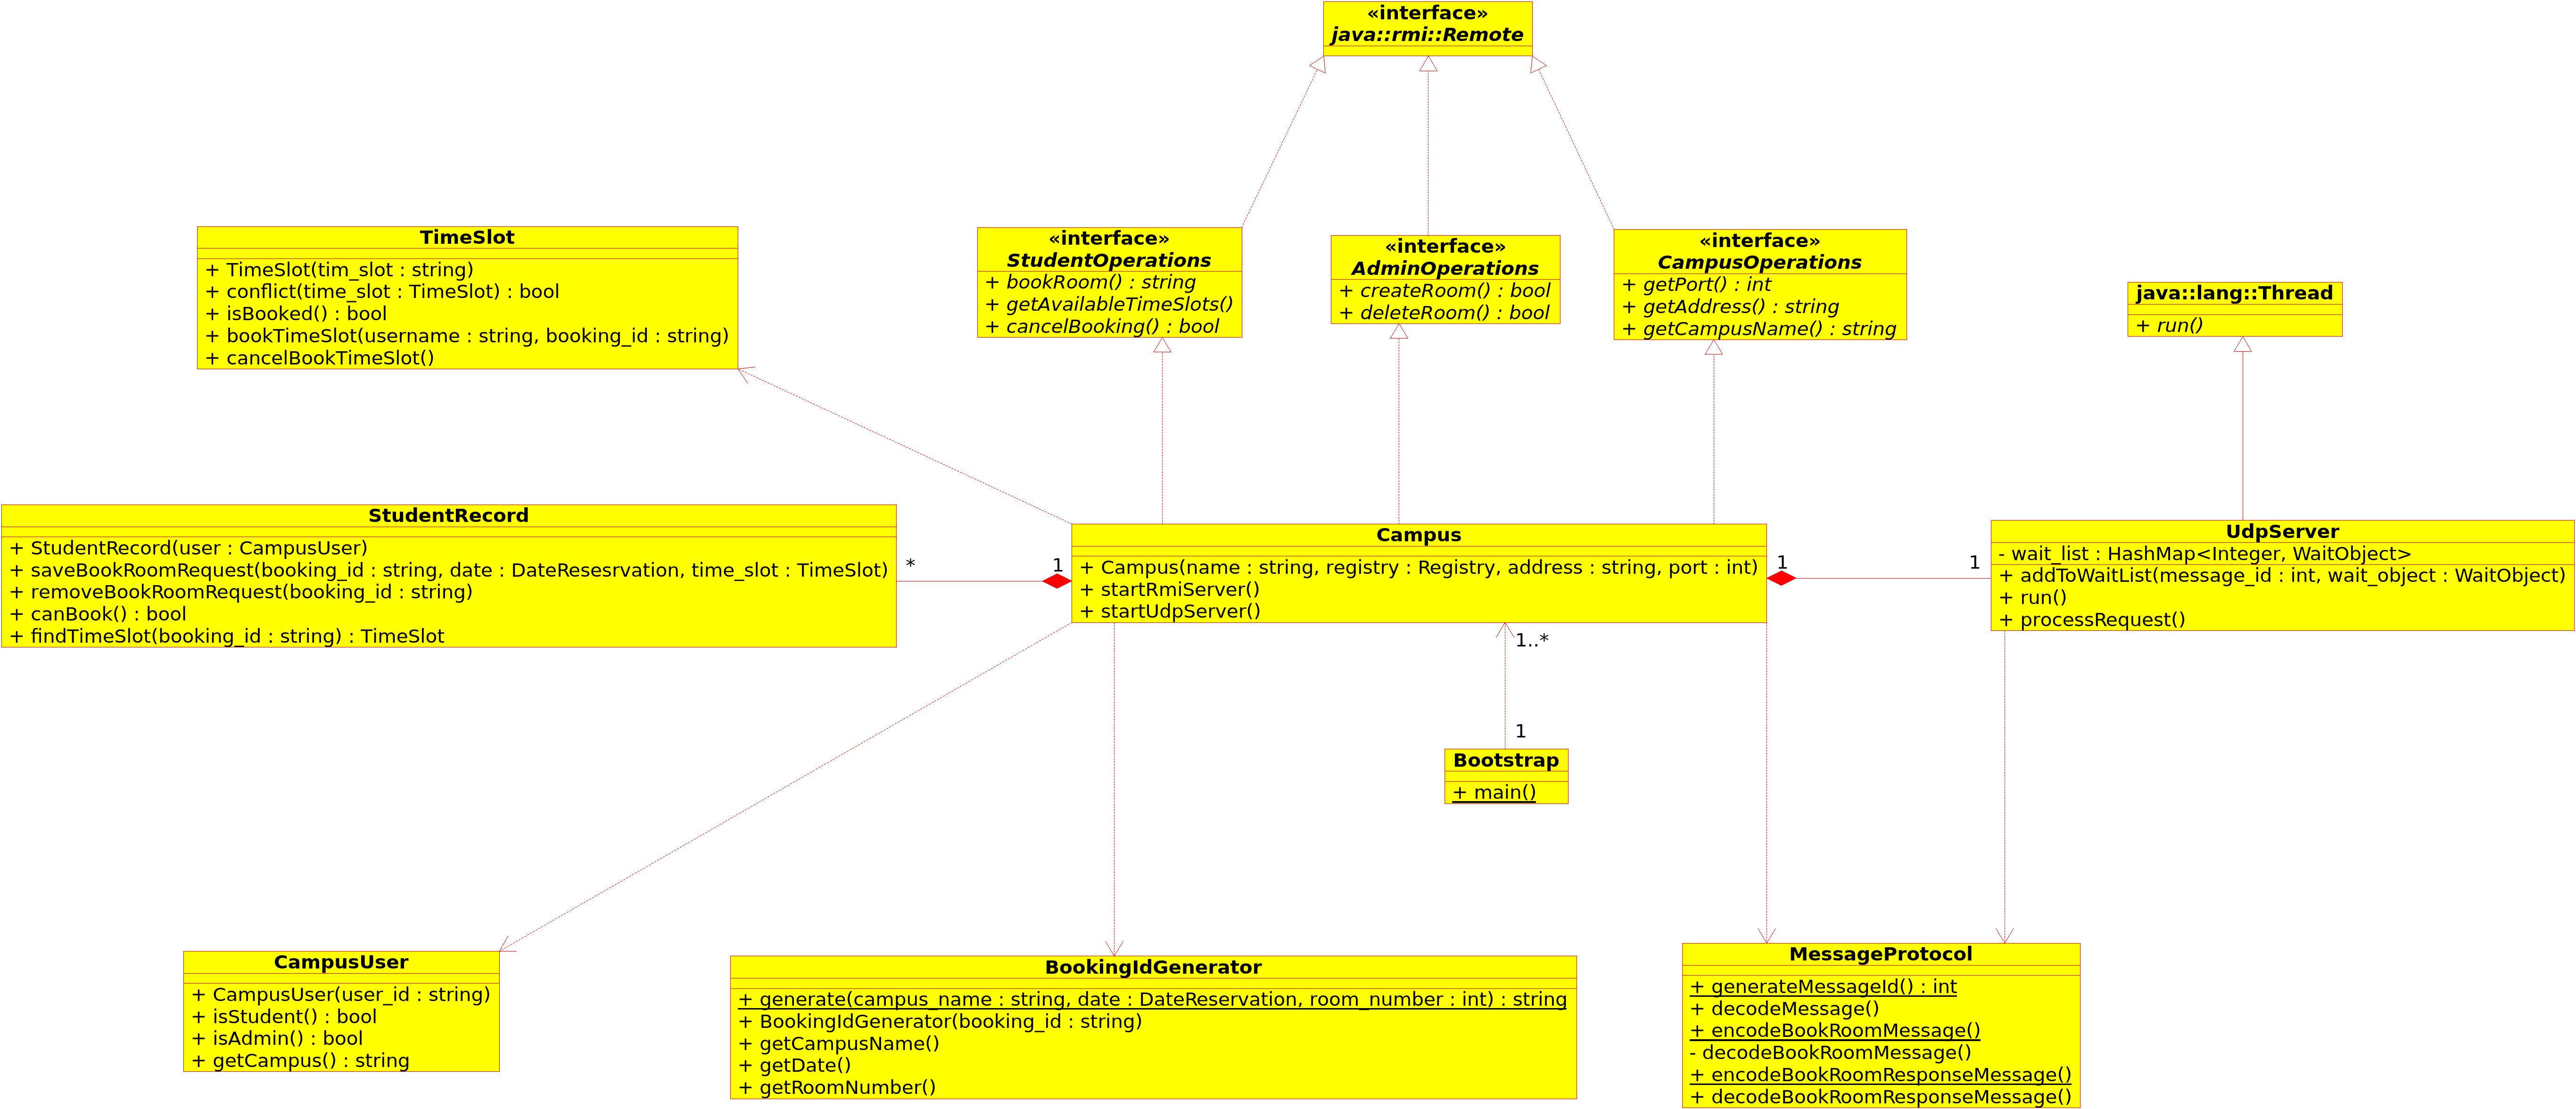
\includegraphics[width=\linewidth]{img/class_diagram.png}
\end{figure}

\par Class $MessageProtocol$ is responsible for my simple text-based protocol. Whenever the campus decided to communicate with another campus, it uses this class to create a message for sending over UDP socket. On the other hand the receiver campus uses this class to decode the string message into POJOs. Every message has a header and a body. The header consists of two fields: message type and message id. Message id is unique in each campus and by using that the campus can determine which student is corresponding to the message. Since each request has a different message format, I use message type to inform the receiver how to parse the message. 
\par As you can see there are some utility classes. All student activities are stored in a $StudentRecord$ object. $BookingIdGenerator$ is responsible for generating a booking id in such a way that we can extract campus name, reservation date and room number from it. $CampusUser$ class can extract the type of user (student or admin) and the campus which user belongs to, from user ID. I also developed a class named $TimeSlot$ which stores the time slot and booking information.

\section{Synchronization}
According to Java SE 8 documentation \cite{hashmap}: "if multiple threads access a hash map concurrently, and at least one of the threads modifies the map structurally, it must be synchronized externally. (A structural modification is any operation that adds or deletes one or more mappings; merely changing the value associated with a key that an instance already contains is not a structural modification.). This is typically accomplished by synchronizing on some object that naturally encapsulates the map". So it is not safe to use $HashMap.get$ when another thread try to change $HashMap$'s structure \cite{hashmap-multithread-get}. I should mention that $HashMap$ is not thread-safe for different keys \cite{hashmap-multithread-different-keys}.
\subsection{Main Database}
I designed three types of object locks for handling $HashMap$ database for multi-threaded environment. One locks the first key (date of reservation), the other locks the second key (room number) and the third locks a list of time slots for a specific date and room number.
\par I've noticed $createRoom$ is similar to $deleteRoom$ but some operations are different. For handling that I design a system which is used in event-handling system. I define a private method named $traverseDb$ which handles all synchronization when we traverse the database and call some abstract methods for handling the differences between $createRoom$ and $deleteRoom$ operations. In other words, those methods should implement abstract class define in listing \ref{lst:DbOperations}. I removed the arguments and the return value for simplicity. As you can see all of them are thread-safe (unless we try to access another database or container). In other words, $createRoom$ and $deleteRoom$ should only implement these thread-safe callbacks. Handling the synchronization is done in $traverseDb$ method.

\begin{lstlisting}[language=java,label={lst:DbOperations},caption={DbOperations abstract class},numbers=left]
private abstract class DbOperations
{
  //All the following methods 
  //are thread-safe for campus time slots database
  public abstract onNullValue();
  public abstract onNullSubValue();
  public abstract void onSubValue();
}
\end{lstlisting}

\par You can see a snippet of $traverseDb$ method implementation in listing \ref{lst:traverse_db}. It is important to put lines 2 - 8 in a $synchronization$ block. In $createRoom$ method it implements $onNullValue$ by creating a new $HashMap$ for room number and list of time slots. If more than one thread try to execute it, each of them has their own new $HashMap$ of room number and list of time slots which is not correct because one of them has stale value.

\begin{lstlisting}[language=java,label={lst:traverse_db},caption={Snippet from traverseDb method},numbers=left]
synchronized (date_db_lock) {
  val = db.get(date);
  if (val == null)
  {
    val = db_ops.onNullValue();
    if (val == null)
      return;
    db.put(date, val);
  }
}		
\end{lstlisting}

\par According to problem statement, we need to update student record when we delete a time slot which that user has booked. I create thread for every time slot which is booked by a user from another campus which is responsible to get notification about the status of student record update from another campus. At the end of method I'm waiting for all created threads to finish their job.

\subsection{Student Database}
This database store the records of a particular student reservation and make sure it does not exceed 3 times per week. I follow the same pattern as main database. I've noticed $bookRoom$ and $cancelBooking$ have a lot in common. So I created a private method named $traverseStudentDb$ which handles traversing student database and calls some callbacks which are implemented differently in $bookRoom$ and $cancelBooking$ methods. You can see the abstract class which both methods should implement in listing \ref{lst:traverse_student_db}. All these methods are thread-safe, unless we want to access another database or container.

\begin{lstlisting}[language=java,label={lst:traverse_student_db},caption={UserDbOperations Abstract Class},numbers=left]
private abstract class UserDbOperations
{
  //All the following methods are tread-safe for user database
  public abstract boolean onUserBelongHere(record);
  public abstract StudentRecord onNullUserRecord(user);
  public abstract boolean onOperationOnThisCampus(time_slots);
  public abstract void onOperationOnOtherCampus(message_id); 
  public abstract void onPostUserBelongHere(record);
  public abstract ArrayList<TimeSlot> findTimeSlots();
}
\end{lstlisting}

\par I also try to lock student's record during the transaction. For example when user wants to book a room on another campus, the student record should be lock until we received answer through UDP communication. When the campus send booking request to another campus, it create a $WaitObject$ object and then calls its $wait$ method. It's the responsibility of UDP server to notify it that its response has arrived.

\subsubsection{Getting Information About Available Time Slots}
This method is different from $bookRoom$ and $cancelBooking$ methods. So it doesn't use $traverseStudentDb$ method. You can see a simple pseudocode in algorithm \ref{algorithm:available-time-slots}. As you can see we need two functions $F$ and $G$ for handling this method. Function $F$ tries to obtain the available time slots in this campus and function $G$ tries in other campus through UDP.

\begin{algorithm}
\caption{Pseudocode For Available Time Slots}
\label{algorithm:available-time-slots}
\begin{algorithmic}[1]
\Function{get-available-timeslos}{date}
\State $S = \Call{F}{date}$
\ForAll{$c \in \{Campuses\} - \{this\_campus\}$}
\State $S = S \cup \Call{G}{c, date}$
\EndFor
\EndFunction
\end{algorithmic}
\end{algorithm}

\par Since we don't know which campus response arrives first, I defined "the number of campuses minus 1" threads (in this assignment 2) which are responsible for extracting information from its corresponding campus. At the end of function I wait for all created threads to finish their job and combine the results and return it to the user.

\subsection{Container Synchronization}
According to $ArrayList$ documentation \cite{ArrayList}: " If multiple threads access an ArrayList instance concurrently, and at least one of the threads modifies the list structurally, it must be synchronized externally. (A structural modification is any operation that adds or deletes one or more elements, or explicitly resizes the backing array; merely setting the value of an element is not a structural modification.) This is typically accomplished by synchronizing on some object that naturally encapsulates the list.". So I need to synchronize accessing $ArrayList$ (or other collections) when I want to access an element or traverse it. According to $Collections$ documentation \cite{Collections}: "It is imperative that the user manually synchronize on the returned list when iterating over it (see listing \ref{lst:collections-sync})".

\subsection{Socket Synchronization}
It is safe to have two threads which one of them read from socket and the other write into it concurrently \cite{socket-full-duplex}. I only have one reader thread so I don't need to do synchronization here. But I can have multiple thread for writing into socket so synchronization is necessary.

\begin{lstlisting}[language=java,label={lst:collections-sync},caption={Collections Synchronization},numbers=left]
List list = Collections.synchronizedList(new ArrayList());
    ...
synchronized (list) {
  Iterator i = list.iterator(); // Must be in synchronized block
  while (i.hasNext())
    foo(i.next());
}
\end{lstlisting}

\section{Testing Scenario}
I've utilized JUnit for testing simple scenarios. I have a unit test for all student and admin operations. I tried to test most common situations. For example a user try to book an invalid time slot or a before-booked time slot.
\par First I created multiple time slots in different campuses so I tested the functionality of admin operations completely. I also tried to do admin operations with a student account. All the operations failed as expected. Then I tried to test student operations. I tried to book a room in user's campus and then I tried to book in other campuses and did the same for delete operation. Then I tried to delete a room which the current user booked in other campus for testing this difficult situation. I did a lot of thread synchronization for handling this situation very well.
\section{Conclusion}
As you can see in my document, a lot of parts are related to  thread synchronization which I spent a lot of time to design. It is the most important and difficult part of this assignment. It's not easy to write some unit tests for it. So I read the critical section parts multiple times to see that I handle all concurrent situations. I merged critical section for $createRoom$ and $deleteRoom$ into a single function which calls some callbacks which are implemented differently in those methods to avoid duplication. I revised critical sections multiple times. Since both methods share the same critical section it was easy to apply those changes to those methods. I follow the same pattern for student database.
\par Other parts were trivial. Because they are handled by Operating System or JDK. Another important part was designing a simple text-based protocol for communicating over network. I design a class for it. The protocol is designed in such a way that it can detect duplication datagrams and discard them.
\bibliographystyle{unsrt}
\bibliography{bibs/websites}

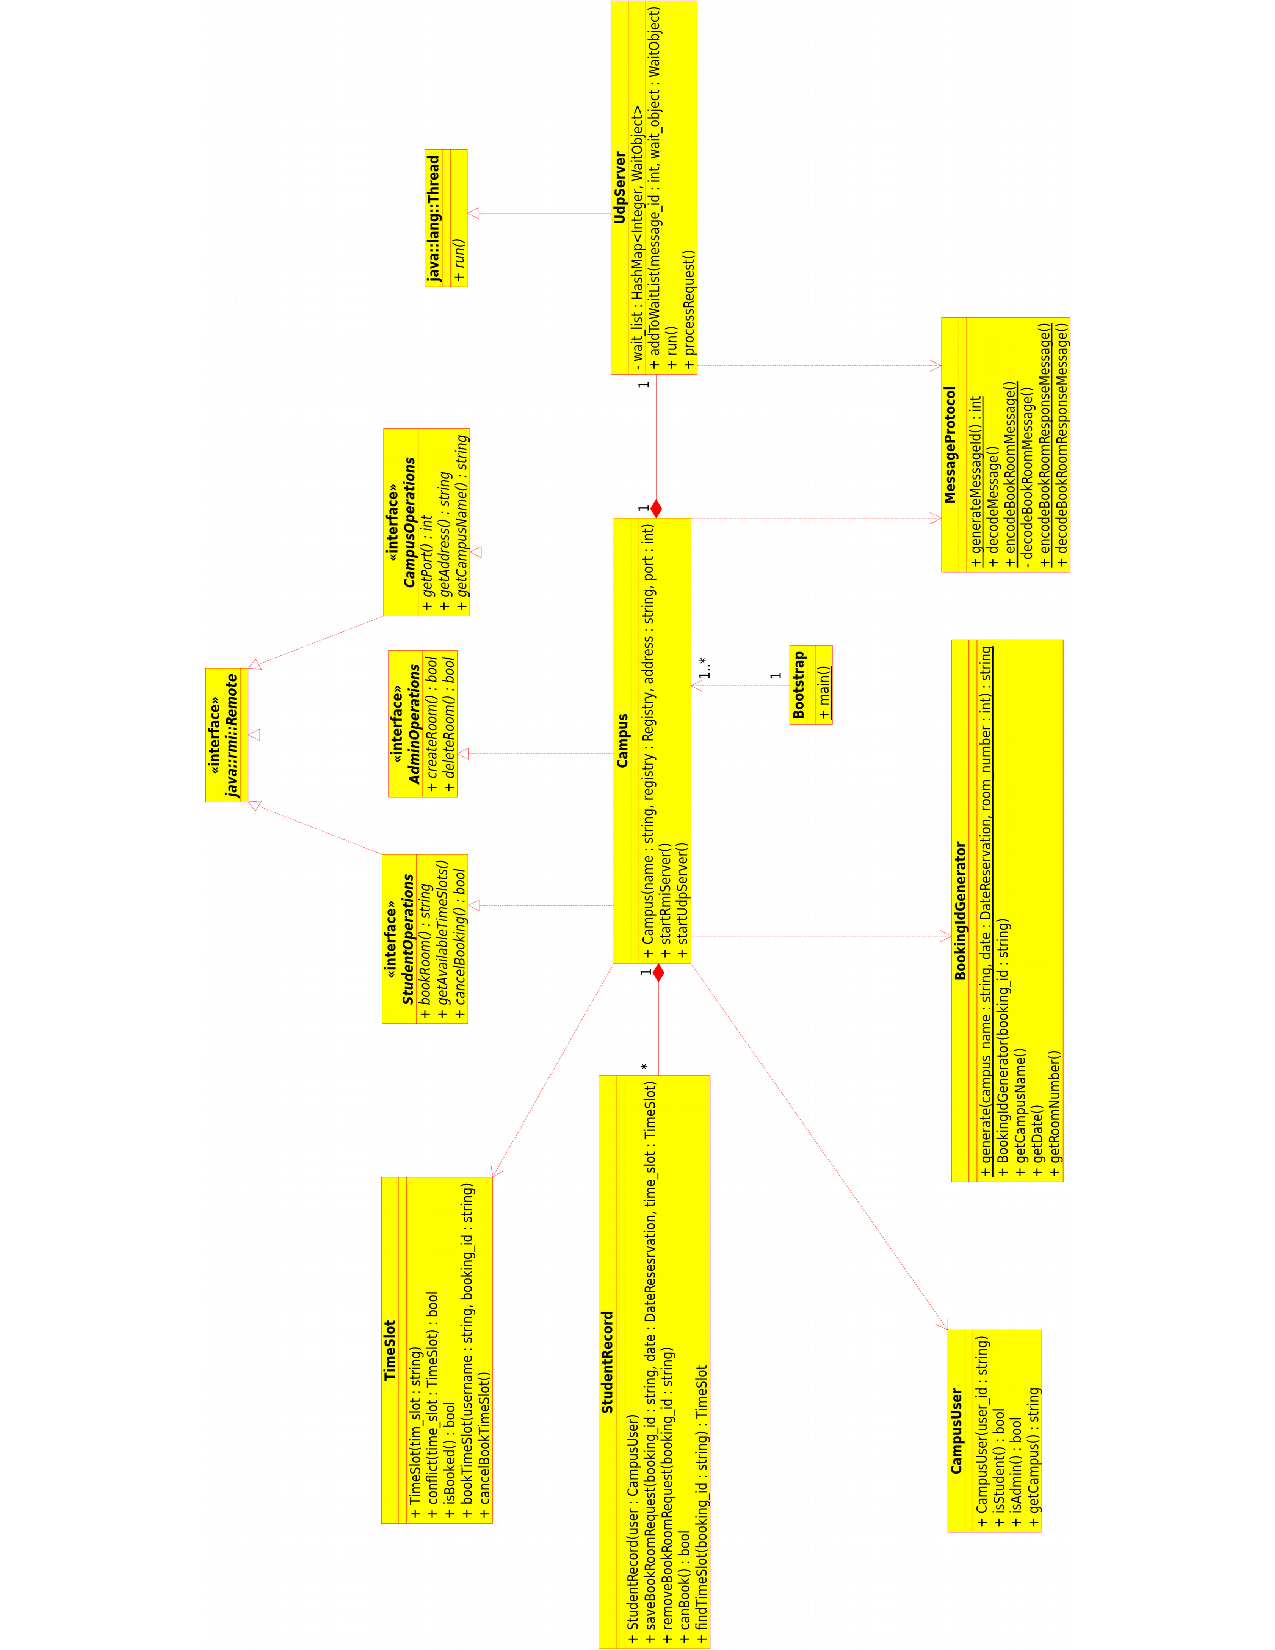
\includepdf[pages={1-}]{class_diagram_page.pdf}
\end{document}
